
\begin{figure}[ht]
  \centering
  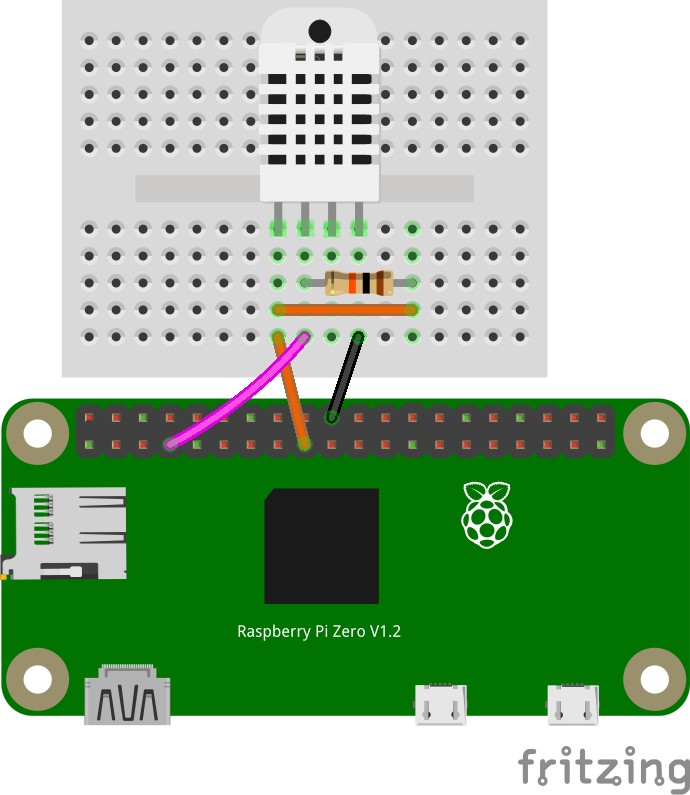
\includegraphics[scale=0.24]{images/DHT22_Steckplatine.png}	
  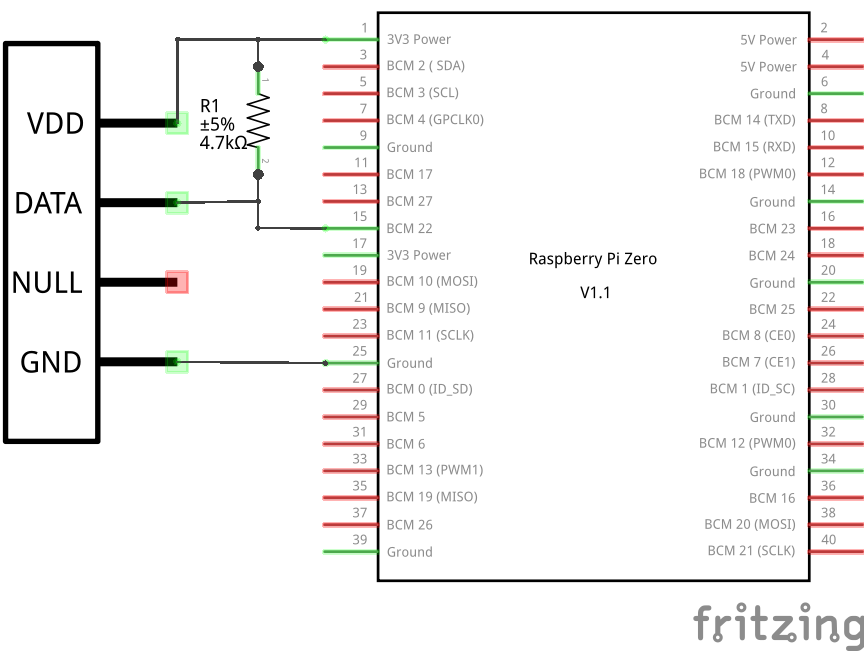
\includegraphics[scale=0.25]{images/DHT22_Schaltplan.png}	
  %	\caption{}
  \label{DHT22_Steckplatine}
\end{figure}


\ExerciseBox{
Lies Temperatur und Feuchte aus [Beispiele]\\
Gib die Werte zyklisch am TM1637 Display aus}


\textbf{C:}

\begin{console}
	git clone https://github.com/mstroh76/Sensors-WiringPi.git
	cd Sensors-WiringPi/DHT
	g++ -o DHT *.cpp -lwiringPi	
	watch -n 2 ./DHT 4
	cd ..
	geany DHT.geany &
\end{console}

\textbf{C\#:}

\begin{console}
	git clone https://github.com/chirndler/wiringpi.net.sensors.git
	cd wiringpi.net.sensors
	xbuild /p:Configuration=Release wiringpi.net.sensors.sln
	cd bin/Release/
	sudo mono wiringpi.net.sensors.sample.exe 1
\end{console}

\textbf{Python:}
% Projektverzeichnis?
\begin{console}
	git clone https://github.com/jdupl/dhtxx-rpi-python3.git
	sudo cp dhtxx-rpi-python3/dhtxx.py /usr/local/lib/python3.5/dist-packages/
\end{console}

\lstset{language=Python, caption=, 
        label=DHT22Program, frame=single, basicstyle=\ttfamily
	      \footnotesize, breakatwhitespace=false, showstringspaces=false, 
        showtabs=false, tabsize=2 }
\lstinputlisting{source/DHT22.py}

\begin{console}
	python3 DHT22.py
\end{console}
